\documentclass[20pt,twocolumn]{article}
\usepackage{geometry}
\geometry{verbose,headsep=3cm,tmargin=2.5cm,bmargin=2.5cm,lmargin=2.0cm,rmargin=2.0cm}
\usepackage{graphicx}
\usepackage{xcolor}
\usepackage[font=small]{caption}
\usepackage{cleveref}
\usepackage{amsmath,amssymb,latexsym}
\usepackage{marvosym}
\usepackage{url}
\usepackage{lipsum}
\usepackage{bm}
\usepackage{float}
\usepackage[english]{babel}
\usepackage{hyperref}
\usepackage{epsf}
\usepackage{float}
\usepackage{mathpazo}
\usepackage{pifont}
\usepackage{wrapfig}
\usepackage{multicol}
\usepackage{enumitem}
\usepackage{xcolor}
\usepackage{framed}
\usepackage[utf8]{inputenc}


\newcommand{\highlight}[1]{%
  \colorbox{orange!50}{$\displaystyle#1$}}

% Document font:
\usepackage{charter}


\begin{document}

\twocolumn[{
\begin{@twocolumnfalse}


  \begin{center}

    \vskip-3em

    \hfill
    \textbf{Bruxelles, November 2018}

    \rule{\textwidth}{0.5pt}
    \vskip2ex

    {\Large\textbf{Underdetermined linear system histograms}}
  
    \vspace{2ex}

      \vspace{1ex}
   
	\texttt{https://camillejr.github.io/science-docs/}
          
  \noindent%
    
\vskip1ex

\rule{\textwidth}{0.5pt}

  \end{center}
  
\vspace{8mm}

\end{@twocolumnfalse}
}]


\vspace{10mm}

\setlength{\parindent}{0cm}


\section{Introduction}

For an undertermined linear system (where matrix $\bm{A}$ is size $(n \times m)$ and $n<m$):

\begin{equation}
\bm{A} x = b
\end{equation}


an infinite number of solutions exists. MATLAB implements various methods of computing possible solutions for $x$. In this paper we investigate the differences in the available solutions by analyzing their histograms. Four methods were selected: backslash \texttt{\char`\\} operator, computing a pseudo-inverse \texttt{pinv()}, and two least-squares algorithms \texttt{lsqnonneg()} and \texttt{lsqr()}.

\section{Matlab example}

We focus on an example where matrix $\bm{A}$ is size $(100 \times 500)$ and a vector $b$ is size $(100 \times 1)$; both are populated by normally distributed random numbers.

\begin{figure}[H]
\centering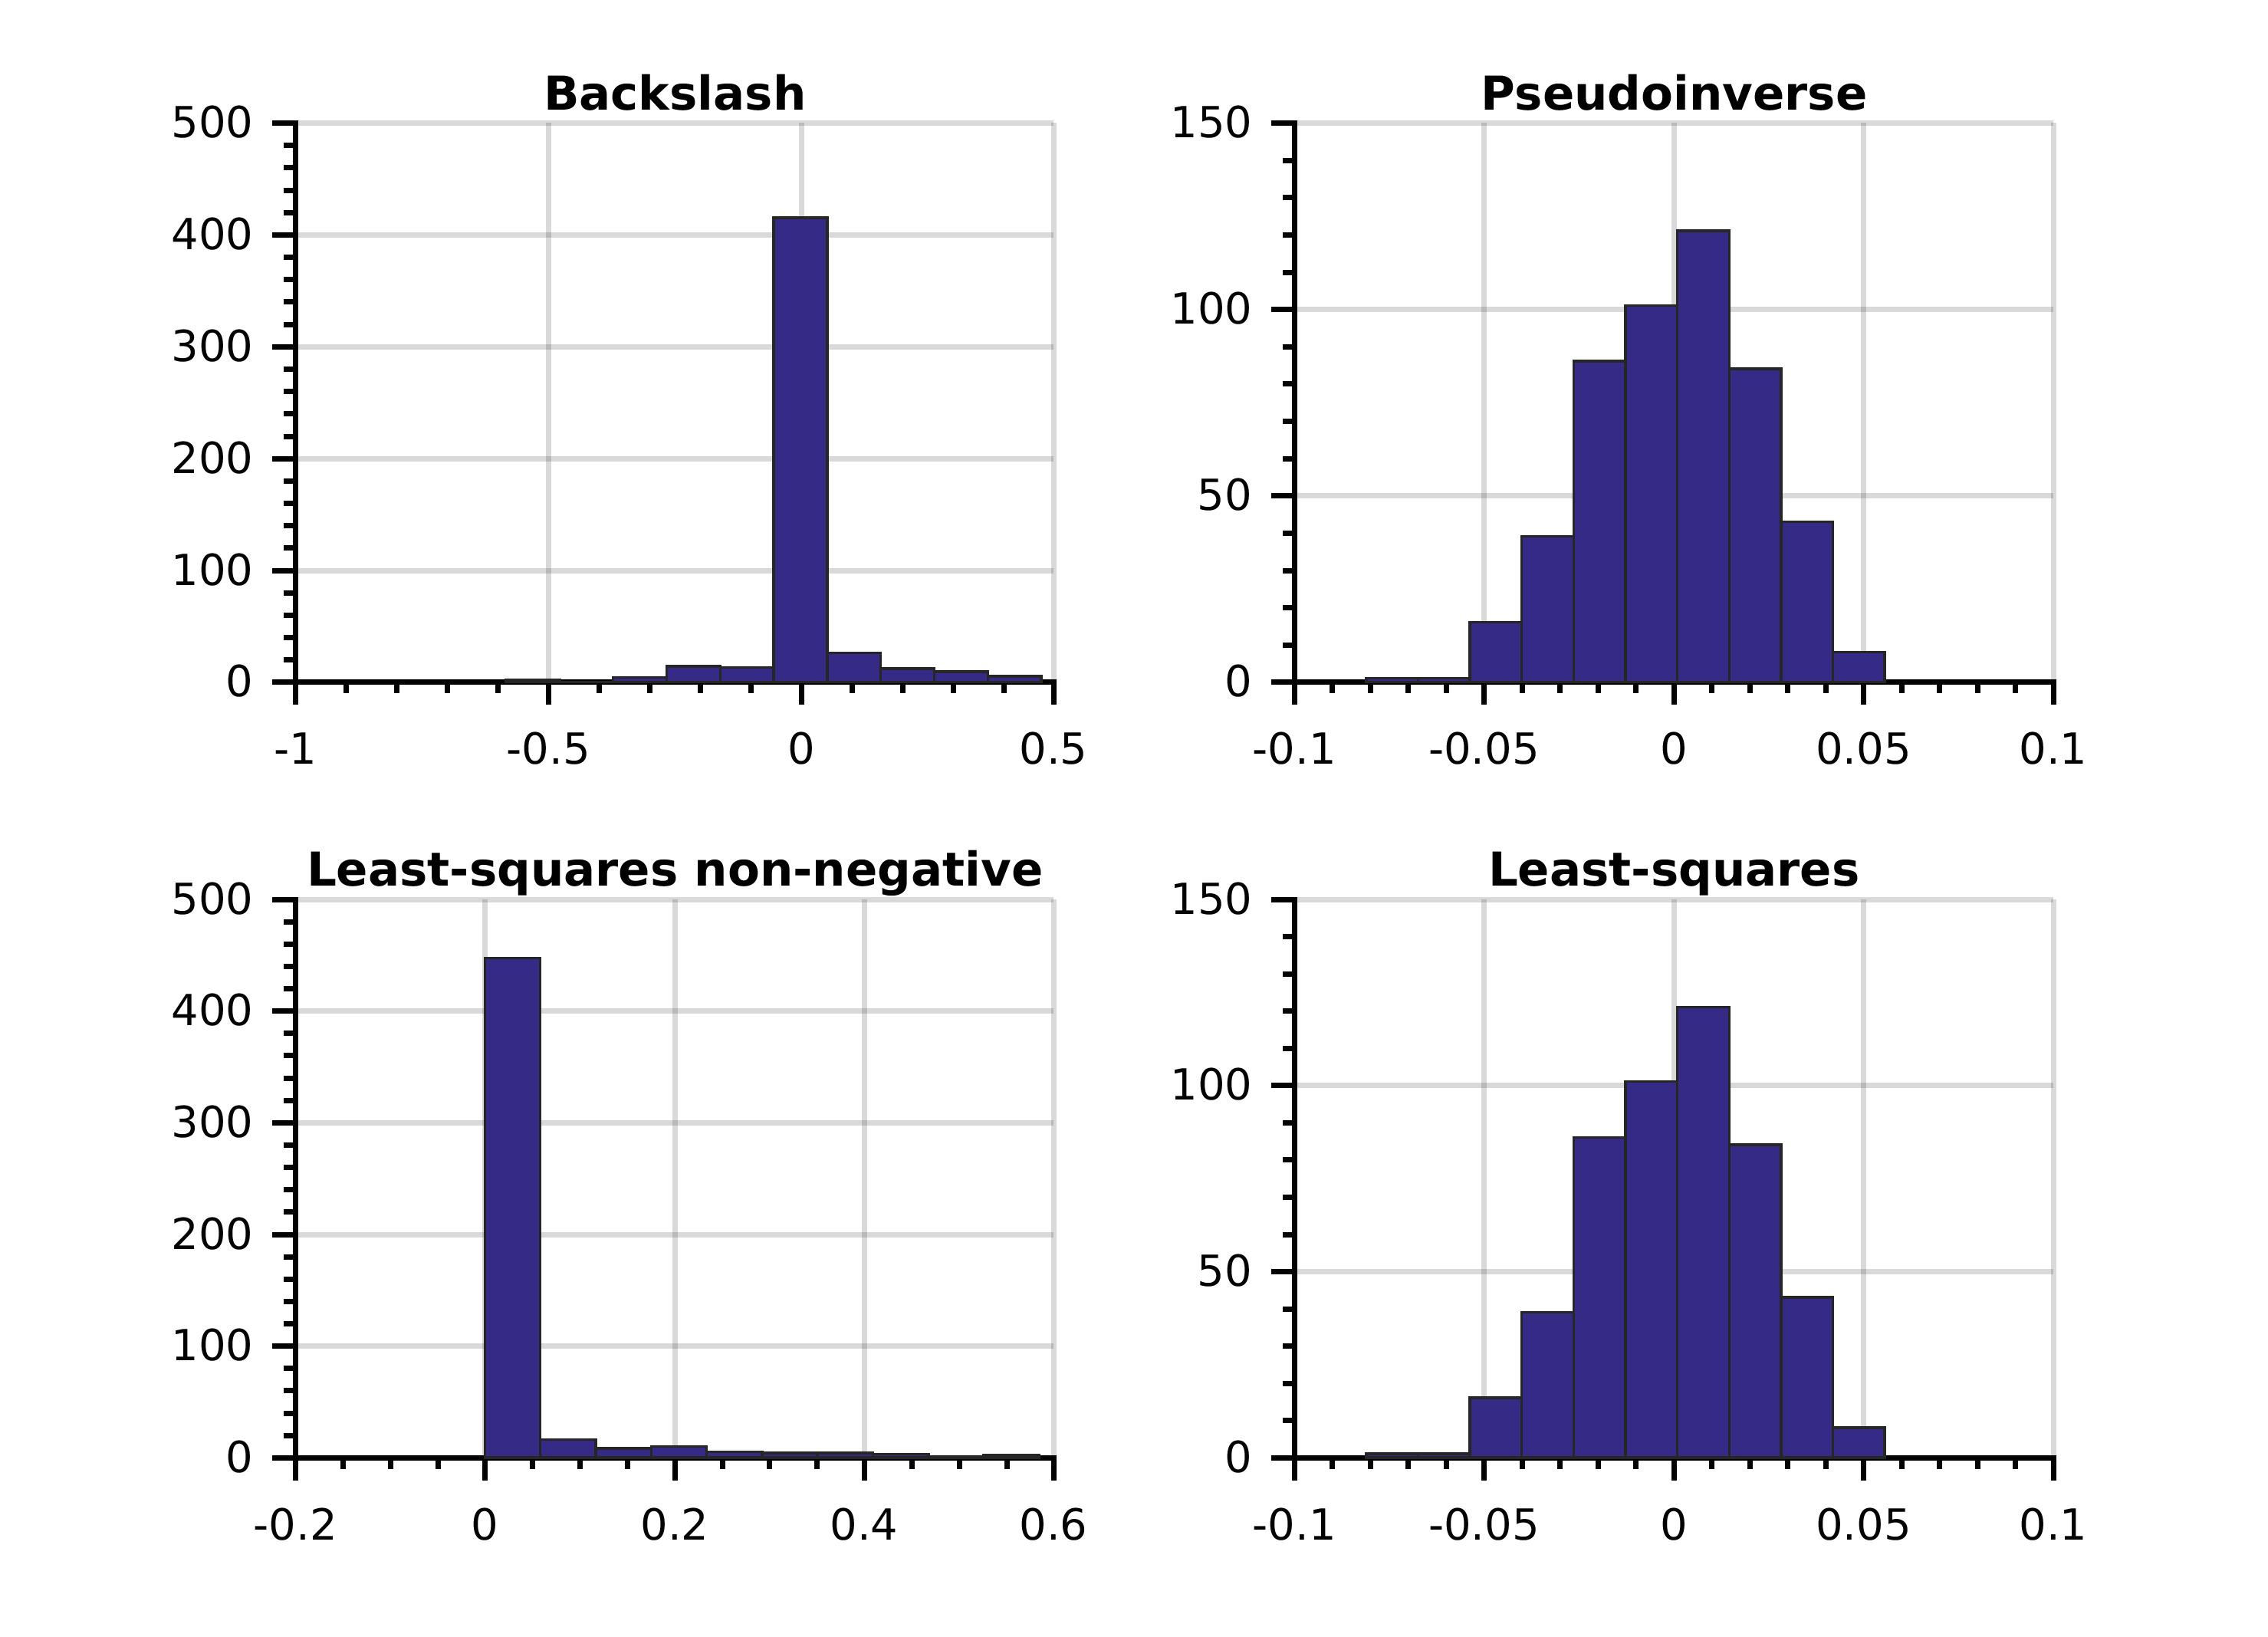
\includegraphics[width=10cm]{DWGs/histograms.png}
\caption{Histograms of four solutions to an undetermined linear system.}			
\label{fig:histograms}
\end{figure}







\section{Possible applications}












\thebibliography{}

\bibitem{Kutz} Nathan Kutz, \textit{Data Driven Discovery of Dynamical Systems and PDEs}, an online lecture 

\bibitem{Strang} Gilbert Strang, \textit{Introduction to Linear Algebra}, Fifth Edition, 2016

 \label{bib:pope}


\end{document}
